% Stanford University PhD thesis style -- modifications to the report style
% This is unofficial so you should always double check against the
% Registrar's office rules
% See http://library.stanford.edu/research/bibliography-management/latex-and-bibtex
% 
% Example of use below
% See the suthesis-2e.sty file for documentation
%
\documentclass{report}
\usepackage{suthesis-2e}
\usepackage{graphicx}
\usepackage{verbatim} % for block comment
\usepackage{color}   % May be necessary if you want to color links
\usepackage{hyperref}
\usepackage{textcomp}
\usepackage{dblfloatfix}
\usepackage[backend=bibtex,style=ieee,natbib=true]{biblatex} % Use the bibtex backend with the authoryear citation style (which resembles APA)
\addbibresource{../src/mybib.bib} % The filename of the bibliography
\hypersetup{
colorlinks=false, %set true if you want colored links
linktoc=all,     %set to all if you want both sections and subsections linked
linkcolor=black,  %choose some color if you want links to stand out
}
\dept{Electronic and Information Engineering}

\begin{document}
    \title{Fast Depth Coding in 3D-HEVC\\
    Using Deep Learning}
    \author{Zhen-xiang WANG}
    \principaladviser{Yui-Lam Chan}
    \beforepreface
    \prefacesection{Abstract}
    The 3D Extension of the High Efficiency Video Coding standard (3D-HEVC),
    which has been finalized by the Joint Collaborative Team on Video Coding
    (JCT-VC) in February 2015, is the new industry standard for 3D applications.
    The 3D-HEVC provides plenty of advanced coding tools specifically
    for addressing the coding of auto-stereoscopic videos which have the format
    of multiple texture views along with the depth maps which are responsible
    for synthesising intermediate views with sufficient quality for
    auto-stereoscopic display.
    The provided tools take advantage of the statistical redundancies amongst
    texture views and depth maps in the video sequences, as well as the unique
    characteristics of depth maps to significantly shrink the bit-rate
    while preserving the objective visual quality of the
    3D videos.
    However, those tools with high capability in terms of compression come
    with the high complexity of computation which has made the encoding time
    of the 3D video sequences much longer than ever by traversing a lot more
    candidates, calculating time-consuming RD Cost for each of them,
    especially in the wedgelet searching process for depth maps.
    While this full-search style method can promise to find the best
    candidate in depth intra mode decision, the time cost is expensive.\\
    \newline
    In this dissertation we address the time cost by presenting a new
    intra mode decision method for depth maps, leveraging the deep
    convolutional neural networks to predict the wedgelet angles
    for the depth blocks.
    The predictions from the learned models are capable of
    reducing the number of wedgelet candidates by half as well as the
    angular modes in depth map coding.
    The size of the neural network has been carefully designed to balance
    the trade-off between the time cost of model prediction and the model prediction
    accuracy.
    Confusion matrix is used to monitor the training process.
    Top-K criteria is employed for the prediction.
    We have integrated the learned models into the reference software of
    3D-HEVC for the experiments.
    The compiled executable binaries are able to harness
    the power of the simultaneous computation of CPU, as well as
    the parrallel computation of GPU to accelerate the predictions.
    The simulation results show that the proposed algorithm
    provides 64.6\% time reduction in average while the
    BD performance has a tiny decrease comparing with the state-of-the-art 3D-HEVC
    standard.

    \prefacesection{Acknowledgments}
%    I would not be able to accomplish the work in this dissertation
%    if it were not for the help
%    from people.
    Allow me first to give sincere thanks to my supervisor,
    Dr.Yui-Lam Chan, for his
    extremely generous support, most insightful advices and innumerable yet
    constructive feedback.
    I learned from him to first identify a problem,
    by reading a vast amount of articles
    to know what people have achieved and what bottlenecks they have encountered.
    I learned how to read papers, how to organize them to
    become the inner comprehension.
    He guided me to use the machine learning approach to solve the
    problem that has been found in the first stage.
    Without his guidance I will not have the idea to learn the deep
    learning technology and apply it to optimize the video coding.
    His encyclopedic knowledge and charming personalities made him my mentor in
    both research and life.
    I wish to thank Dr.Sik-Ho Tsang, for our in-depth discussions from
    which I can always find useful clues to proceed to next step.
    His great expertise in video coding significantly benefits me during my
    intensive period of learning.
    Also I would like to thank my friends Alex
    and Jacky, for our
    extensive discussions about artificial intelligence
    and their applications.
    Finally thank you my parents, for the great love and constant
    encouragement which give me confidence to face and handle all the
    challenges at every moment.
    \afterpreface

    \chapter{Introduction}\label{ch:chapter1} % For referencing the chapter elsewhere, use \ref{Chapter1}

%----------------------------------------------------------------------------------------
Video is the medium to record, copy, playback, broadcast
and display the motion images in an electronic style~\parencite{RN190}.
Watching videos is becoming an important way for our entertainment as well
as education.
The high definition (HD) and ultra high definition (UHD) video
are increasingly demanding nowadays.
People prefer videos with higher definitions than those with lower
resolutions because the former one provides much better viewing experience.
However, challenges emerged for delivering videos with high definition.
HD videos typically contain much more information in every picture frame than the
standard definition videos.
More data needs to be squeezed into the same capacity for transmission.
For example, the uncompressed video with the dimension 720 x 480 at 30 frames
per second requires 0.03 gigabytes per second, while the uncompressed video with
the dimension 2880 x 2048 at 120 frames per second requires 2.12 gigabytes per
second.
Since bit rate is proportional to system bandwidth for
transmission~\parencite{RN191}, and expanding the bandwidth in a large scale is
too expensive, the significantly increased bit rate
for transmitting the video data is becoming one of the
major obstacles for HD video services.\\
\newline
To cope with the growing need for higher compression of moving
pictures~\parencite{RN193}, Joint Collaborative Team on Video
Coding (JCT-VC)~\parencite{RN192} has developed the High Efficiency Video
Coding standard which is the newest international video coding standard for
substantially ameliorate the compression performance against the previous
standards.
Comparing with the H.264 Advanced Video Compression Standard~\parencite{RN194},
the H.265 High Efficiency Video Coding Standard provides fifty percent bit rate
reduction while maintaining the objective video quality at the same level.\\
\newline
While Two-dimensional video is the most common video type,
Three-dimensional (3D) video has been brought to market via lots of ways,
including Blu-Ray disc, cable and satellite transmission, terrestrial
broadcast, and streaming or downloading from the Internet~\parencite{RN118}.
3D video provides the perception of depth information which augments
the vividness of the video contents.
Currently most 3D videos in the market are using stereo display technology.
Two similar views, one for left eye, the other for right eye, are presented
at the same time with the multiplexing techniques enabling the
adjustments of video geometry information~\parencite{RN196} to provide
the 3D effect.
Figure~\ref{fig:stereo-display} illustrates the typical system structure for
transmitting videos targeting stereo display.
It can be observed that there exists a displacement between the
two views.
The green vertical left margins of the red rectangles in the two views
at encoder side are different.
Such a displacement is the visual disparity for 3D perception.
Stereoscopic videos~\parencite{RN153} have
achieved great profitability for movie theatres in recent years.
For example, IMAX 3D has became the most popular one that offering
the immersing multimedia experiences around the world.
Special 3D glasses are needed for watching the IMAX 3D movies.
The current 3D film industry is very successful in terms of attracting
customers, however, it is not the end of the story.
Myopic people do not like to wear one more pair of glasses when
watching 3D movies.
Some people will experience discomfort after wearing the 3D glasses for a
period of two hours.
Autostereoscopic multi-view technology~\parencite{RN153} is coming to our rescue.
No glasses are needed if Autostereoscopic videos can
substitute the Stereoscopic videos.
The Autostereoscopic multi-view display demands more than two
views for audience to view the 3D contents
without extra eye glasses.
The visual quality of
the Autostereoscopic display is highly correlated to the number of views
that can be provided in the receiver side.
Due to limited available bandwidth, transmitting arbitrary number of views
is not practical.
Researchers have proposed a new format which is making use of limited number
of view and their associated depth maps~\parencite{RN44}.
The typical system structure for using this new format to compress and supply 3D video
resources is shown in figure~\ref{fig:SS-MVD}.
\begin{figure}
    \centering
    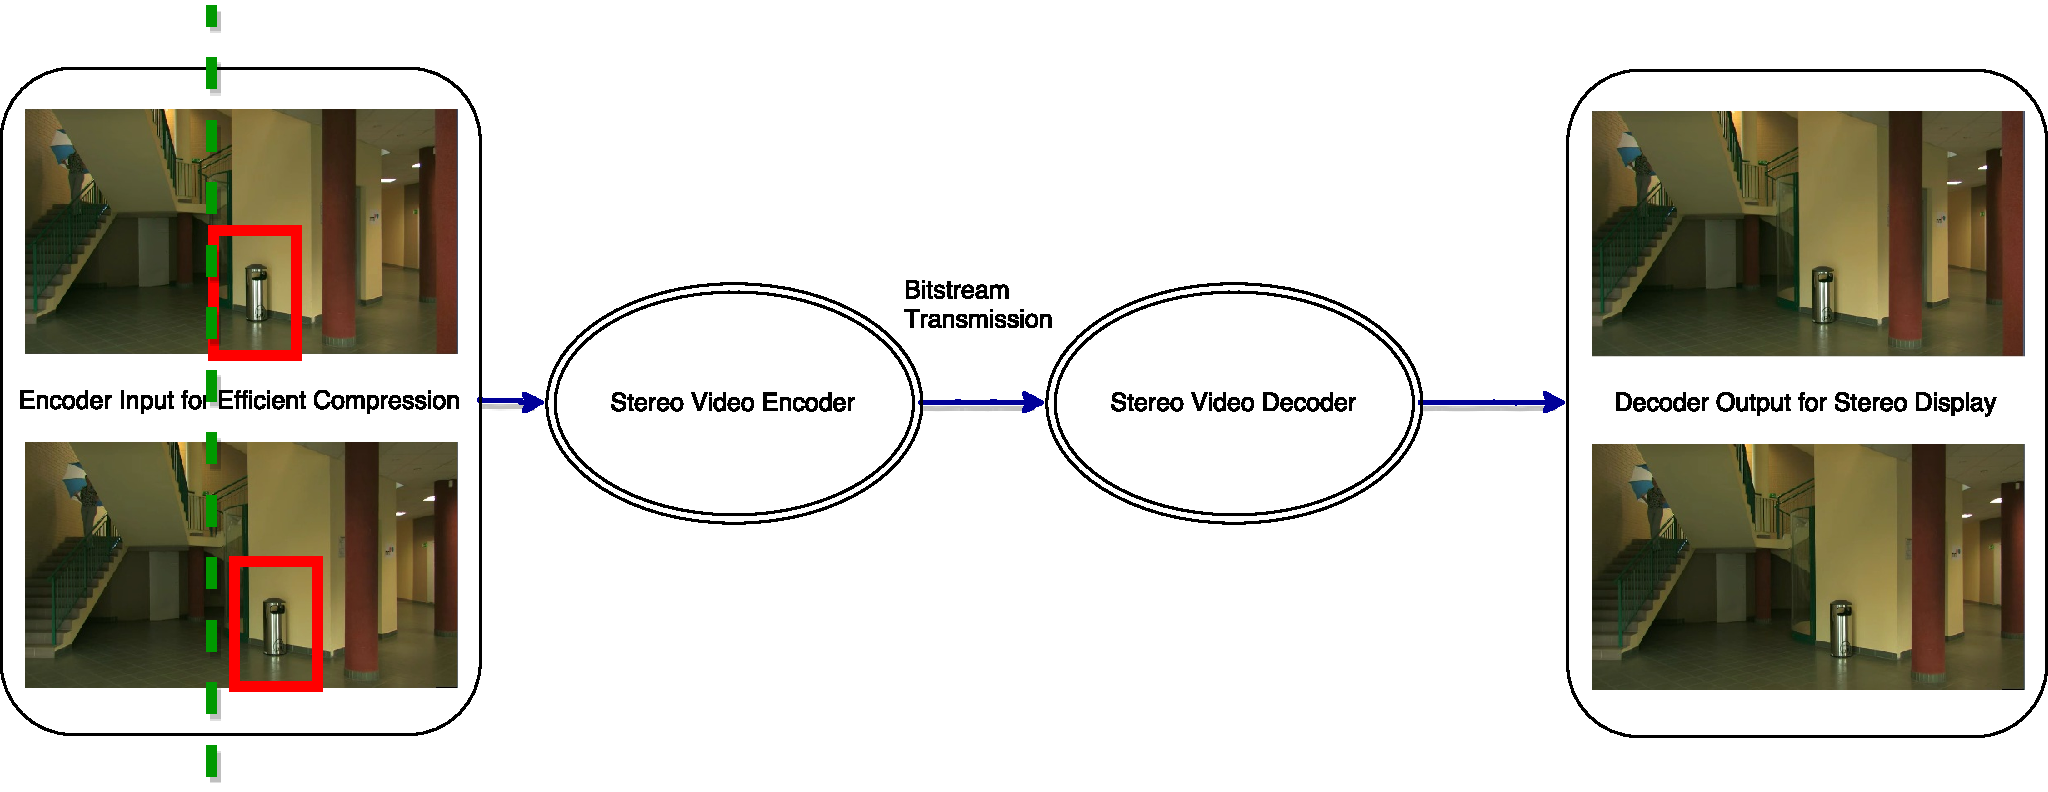
\includegraphics[width=\textwidth,height=\textheight,keepaspectratio]{Figures/StereoDisplay}
%        \decoRule
    \caption[System Structure for transmitting videos targeting stereo display]{System Structure for transmitting videos targeting stereo display.}
    \label{fig:stereo-display}
\end{figure}
An enormous amount of views in the medium positions which are able to
guarantee the high quality of the 3D video can be synthesized from
\begin{figure}
    \centering
    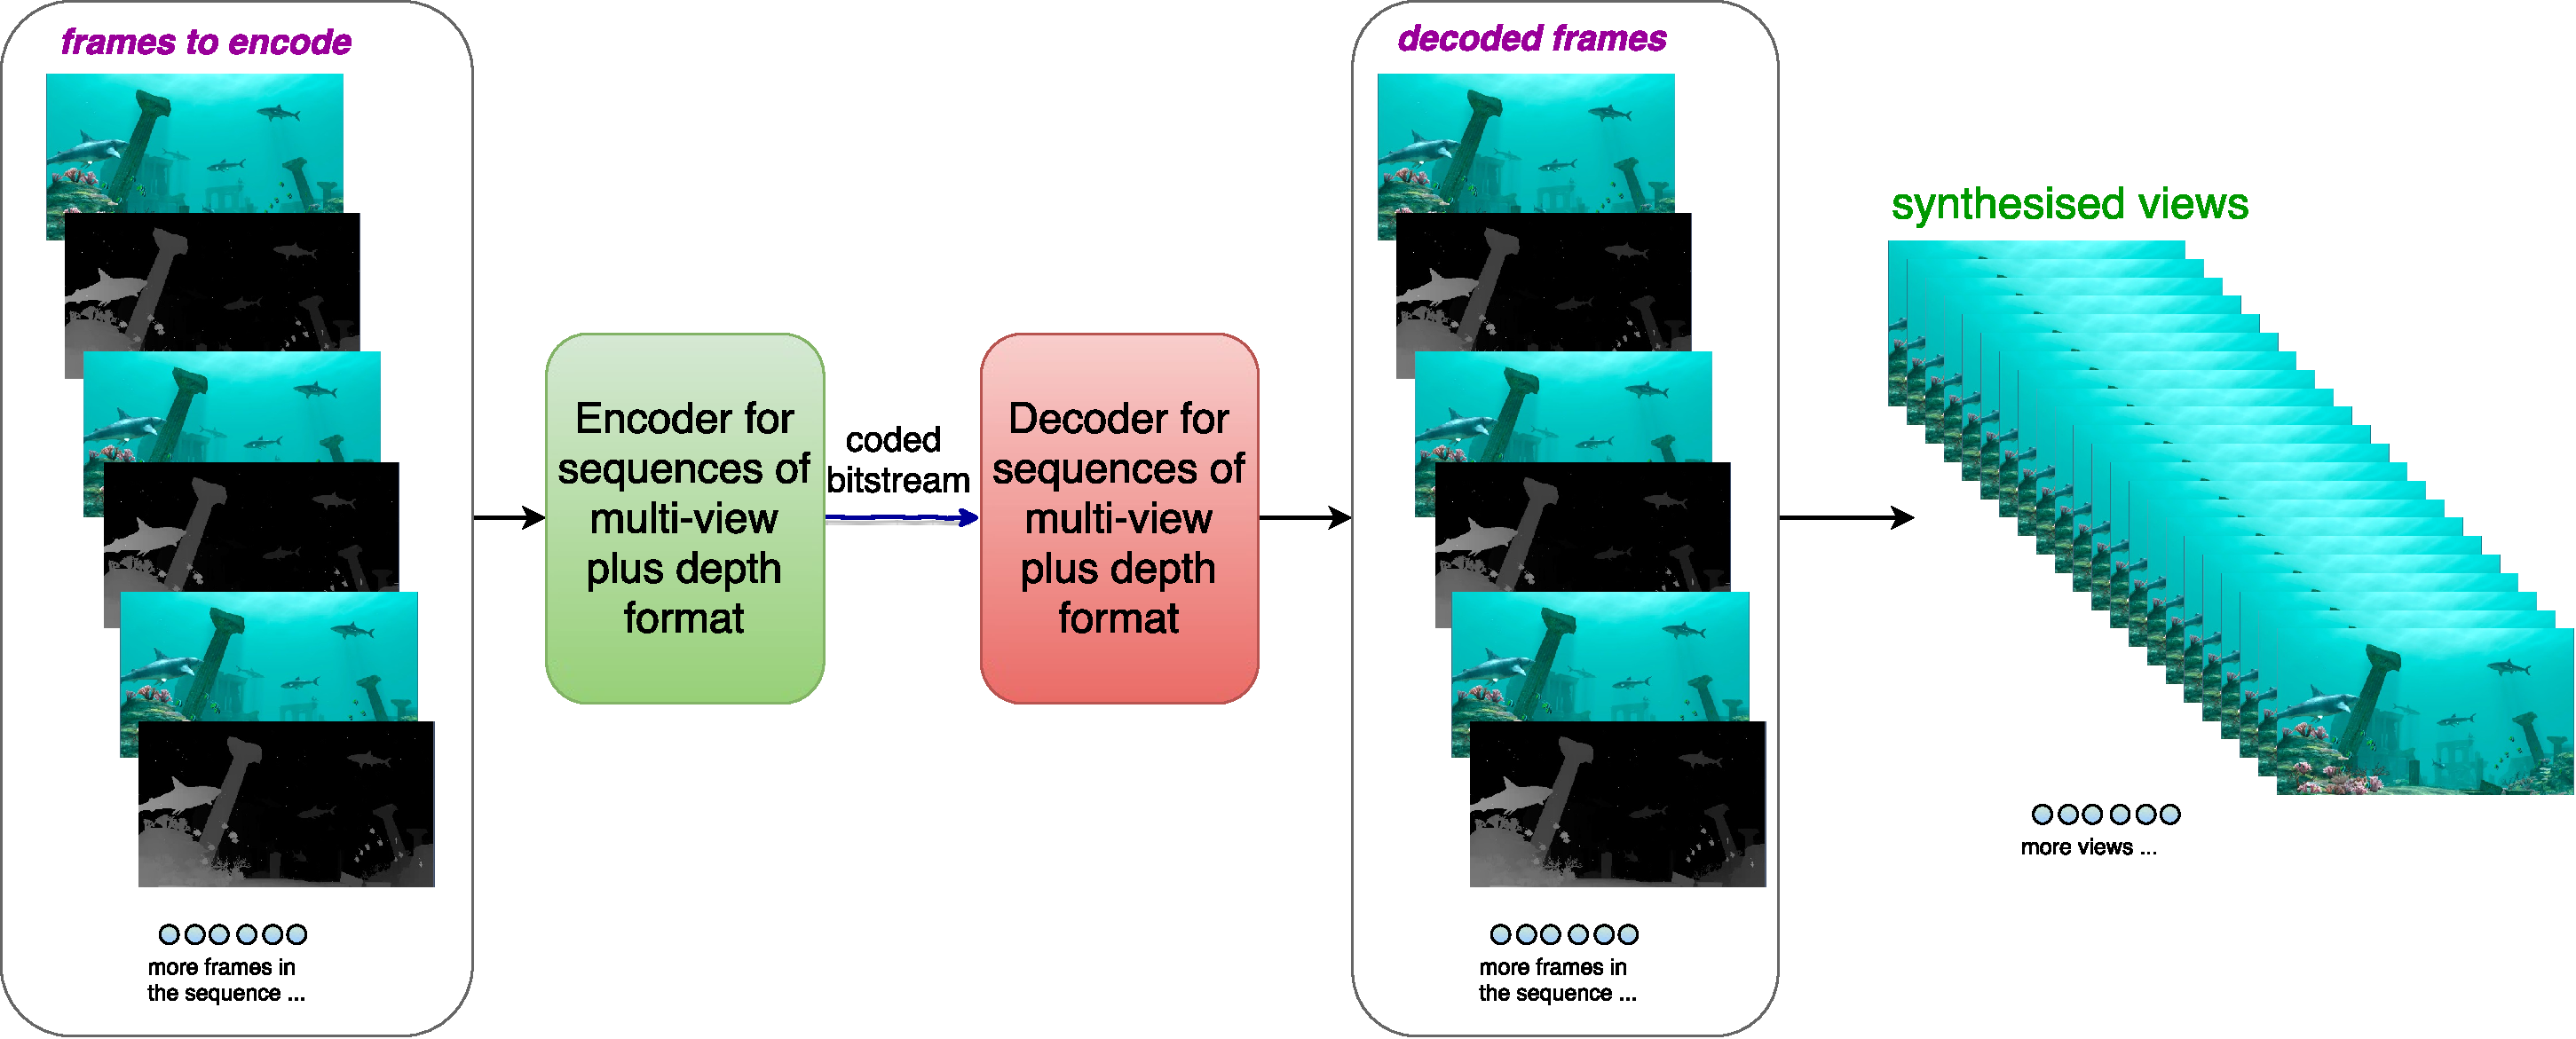
\includegraphics[width=\textwidth,height=\textheight,keepaspectratio]{Figures/SystemStructureOf3DEncoder}
%        \decoRule
    \caption[System Structure for transmitting videos of Multi-view Plus Depth format]{System Structure for transmitting videos of Multi-view Plus Depth format.}
    \label{fig:SS-MVD}
\end{figure}
the decoded texture frames in combination with decoded depth maps.\\
%The multi-view plus depth format provides the functionality of synthesizing
%required number of views from texture views and associated depth maps.\\
\newline
To employ multi-view plus depth format for 3D video, efficient compressing
methods are desired, which has led to the 3D Video Coding Extension of the
High Efficiency Video Coding Standard (3D-HEVC) by the Joint Collaborative Team
on 3D Video Coding Extension Development (JCT-3V)~\parencite{RN195}.
The 3D Extension of the HEVC standard gives extra coding efficiency
for encoding a few texture views along with the corresponding depth maps by
using new tools which exploit the redundancies amongst
texture and depth views, and pay attention to the unique characteristics of
the depth maps, such as large homogeneous
regions separated by sharp boundaries~\parencite{RN47}.\\
\newline
Depth information measures of the distance between the object in the far position
and the object in the near position from a static viewpoint,
which is expressed in the format of depth map.
Instead of presenting depth maps directly to the viewer, views in the medium
positions are generated by Depth-Image-Based Rendering (DIBR) technique.
The qualities of the depth maps are vital to the DIBR process.
Corona artifacts (a.k.a. ringing artifacts) can be discovered in synthesized
views if the edge sharpness in depth maps can not be well
preserved.
Therefore, retaining the edge sharpness in depth map is the key to avoid the
artifacts in the synthesized views.
In 3D-HEVC, new intra-picture prediction and residual coding methods
have been applied to preserve the special properties of depth
map.
Depth Modelling Mode (DMM), which is one of the new intra-picture
prediction tools, is designed to provide much more granularity for
encoding the depth maps.
Wedgelet partition and contour partition for depth maps
are enabled by DMM1 and DMM4 separately.
%~\parencite{RN197}.

%introduce a little about depth map and their usage.
%mentioning iphonex true depth camera.
%draw the picture

%----------------------------------------------------------------------------------------

\section{Motivation and Contribution}\label{sec:motivation_and_contribution}
%fasdfasdfasdfasdfasdfasdf figure~\ref{fig:SS-MVD}
If you are
\begin{table}
    \label{tab:treatments}
    \centering
    \begin{tabular}{c r @{.} l}
        Pi expression       &
        \multicolumn{2}{c}{Value} \\
        \hline
        $\pi$               & 3&1416  \\
        $\pi^{\pi}$         & 36&46   \\
        $(\pi^{\pi})^{\pi}$ & 80662&7 \\
    \end{tabular}
    \caption{The effects of treatments X and Y on the four groups studied.}
\end{table}

\begin{table}
    \label{tab:tabular_example1}
    \centering
    \begin{tabular}[t]{|r|l|}
        \hline
        7C0 & hexadecimal \\
        3700 & octal \\
        \cline{2-2} 11111000000 & binary \\
        \hline
        \hline
        1984 & decimal \\
        \hline
    \end{tabular}
\caption{Just an example}
\end{table}

\begin{table}
    \label{tab:tabular_example2}
    \centering
    \begin{tabular}{|r|l|}
        \hline
        7C0 & hexadecimal \\
        3700 & octal \\
%        \cline{2-2}
%        11111000000 & binary \\
%        \hline
%        \hline
%        1984 & decimal \\
        \hline
    \end{tabular}
\caption{Basic Usage}
\end{table}

\begin{table}
    \label{tab:tabular_example3}
    \centering
    \begin{tabular}{|r|l|}
        \hline
        7C0 & hexadecimal \\
        \cline{1-2}
        3700 & octal \\
        \cline{2-2}
        11111000000 & binary \\
        \cline{1-2}
        11111000 & binary \\
%        \hline
%        \hline
%        1984 & decimal \\
        \hline
    \end{tabular}
\caption{horizontal lines extend over multiple columns}
\end{table}

\begin{table}
    \label{tab:tabular_example4}
    \centering
    \begin{tabular}{|p{4.7cm}|}
        \hline Welcome to Boxy's paragraph. We sincerely hope you'll all enjoy the show.\\
        \hline
    \end{tabular}
    \caption{define a special type of column which will wrap-around the text as in a normal paragraph}
\end{table}

\begin{table}
    \label{tab:tabular_example8}
    \centering
    \begin{tabular}{p{4.7cm}}
        \hline
        Welcome to Boxy's paragraph.
        We sincerely hope you'll all enjoy the show.\\
        \hline
    \end{tabular}
    \caption{define a special type of column which will wrap-around the text as in a normal paragraph}
\end{table}

\begin{table}
    \label{tab:tabular_example5}
    \centering
    \begin{tabular}{@{} l @{}}
        \hline Welcome to Boxy's paragraph. We sincerely hope you'll all enjoy the show.\\
        \hline
    \end{tabular}
    \caption{define a special type of column which will wrap-around the text as in a normal paragraph}
\end{table}

\begin{table}
    \label{tab:tabular_example6}
    \centering
    \begin{tabular}{l}
        \hline Welcome to Boxy's paragraph. We sincerely hope you'll all enjoy the show.\\
        \hline
    \end{tabular}
    \caption{define a special type of column which will wrap-around the text as in a normal paragraph}
\end{table}

\begin{table}
    \label{tab:tabular_example9}
    \centering
    \begin{tabular}{c c} \hline \multicolumn{2}{c}{Ene} \\ \hline Mene & Muh! \\ \hline \end{tabular}
    \caption{multicolumn command}
\end{table}

\begin{table}
    \label{tab:tabular_example10}
    \centering
    \begin{tabular}{c c c c c c}
        \hline
        sequence name &
        BD-BR &
        \multicolumn{4}{c}{Ene} \\
        \cline{3-6}
        {} & {} & Me & Muh & Me & Mu\\
        \hline
        Newspaper & 0.98\% & 22 & 33 & 44 & 66\\
    \end{tabular}
    \caption{multicolumn command}
\end{table}




%\begin{table}
%    \label{tab:treatments}
%    \centering
%    \begin{tabular}{c r @{.} l}
%        Pi expression       &
%        \multicolumn{2}{c}{Value} \\
%        \hline
%        $\pi$               & 3&1416  \\
%        $\pi^{\pi}$         & 36&46   \\
%        $(\pi^{\pi})^{\pi}$ & 80662&7 \\
%    \end{tabular}
%    \caption{The effects of treatments X and Y on the four groups studied.}
%\end{table}
%----------------------------------------------------------------------------------------

\section{Dissertation Outline}\label{sec:outline}




%\chapter{Introduction}\label{ch:chapter1} % For referencing the chapter elsewhere, use \ref{Chapter1}
%
%%----------------------------------------------------------------------------------------
%
%%----------------------------------------------------------------------------------------
%
%\section{Welcome and Thank You}\label{sec:welcome}
%Welcome to this \LaTeX{} Thesis Template, a beautiful and easy to use template for writing a thesis using the \LaTeX{} typesetting system.
%
%If you are writing a thesis (or will be in the future) and its subject is technical or mathematical (though it doesn't have to be), then creating it in \LaTeX{} is highly recommended as a way to make sure you can just get down to the essential writing without having to worry over formatting or wasting time arguing with your word processor.
%
%\LaTeX{} is easily able to~\parencite{RN93} professionally typeset documents that run to hundreds or thousands of pages long. With simple mark-up commands, it automatically sets out the table of contents, margins, page headers and footers and keeps the formatting consistent and beautiful. One of its main strengths is the way it can easily typeset mathematics, even \emph{heavy} mathematics. Even if those equations are the most horribly twisted and most difficult mathematical problems that can only be solved on a super-computer, you can at least count on \LaTeX{} to make them look stunning.
%
%%----------------------------------------------------------------------------------------
%
%\section{Welcome and Thanku}\label{sec:welome}
%Welcome to this \LaTeX{} Thesis Template, a beautiful and easy to use template for writing a thesis using the \LaTeX{} typesetting system.
%
%If you are writing a thesis (or will be in the future) and its subject is technical or mathematical (though it doesn't have to be), then creating it in \LaTeX{} is highly recommended as a way to make sure you can just get down to the essential writing without having to worry over formatting or wasting time arguing with your word processor.
%
%\LaTeX{} is easily able to professionally typeset documents that run to hundreds or thousands of pages long. With simple mark-up commands, it automatically sets out the table of contents, margins, page headers and footers and keeps the formatting consistent and beautiful. One of its main strengths is the way it can easily typeset mathematics, even \emph{heavy} mathematics. Even if those equations are the most horribly twisted and most difficult mathematical problems that can only be solved on a super-computer, you can at least count on \LaTeX{} to make them look stunning.
%
%%----------------------------------------------------------------------------------------
%
%\section{Welcome and ThYou}\label{sec:weome}
%Welcome to this \LaTeX{} Thesis Template~\parencite{Reference1}, a beautiful and easy to use template for writing a thesis using the \LaTeX{} typesetting system.
%
%If you are writing a thesis (or will be in the future) and its subject is technical or mathematical (though it doesn't have to be), then creating it in \LaTeX{} is highly recommended as a way to make sure you can just get down to the essential writing without having to worry over formatting or wasting time arguing with your word processor.
%
%\LaTeX{} is easily able to professionally typeset documents that run to hundreds or thousands of pages long. With simple mark-up commands, it automatically sets out the table of contents, margins, page headers and footers and keeps the formatting consistent and beautiful. One of its main strengths is the way it can easily typeset mathematics, even \emph{heavy} mathematics. Even if those equations are the most horribly twisted and most difficult mathematical problems that can only be solved on a super-computer, you can at least count on \LaTeX{} to make them look stunning.
%
%%----------------------------------------------------------------------------------------
%
%\section{Welcome and Thau}\label{sec:welcoe}
%Welcome to this \LaTeX{} Thesis Template, a beautiful and easy to use template for writing a thesis using the \LaTeX{} typesetting system.
%
%If you are
%\begin{table}
%
%    \label{tab:treatments}
%    \centering
%%    \begin{tabular}{l l l}
%%        \toprule
%%        \tabhead{Groups} & \tabhead{Treatment X} & \tabhead{Treatment Y} \\
%%        \midrule
%%        1 & 0.2 & 0.8\\
%%        2 & 0.17 & 0.7\\
%%        3 & 0.24 & 0.75\\
%%        4 & 0.68 & 0.3\\
%%        \bottomrule\\
%%    \end{tabular}
%    \begin{tabular}{c r @{.} l}
%        Pi expression       &
%        \multicolumn{2}{c}{Value} \\
%        \hline
%        $\pi$               & 3&1416  \\
%        $\pi^{\pi}$         & 36&46   \\
%        $(\pi^{\pi})^{\pi}$ & 80662&7 \\
%    \end{tabular}
%    \caption{The effects of treatments X and Y on the four groups studied.}
%\end{table}
%writing a thesis (or will be in the future) and its subject is technical or mathematical (though it doesn't have to be), then creating it in \LaTeX{} is highly recommended as a way to make sure you can just get down to the essential writing without having to worry over formatting or wasting time arguing with your word processor.
%
%\LaTeX{} is easily able to professionally typeset documents that run to hundreds or thousands of pages long. With simple mark-up commands, it automatically sets out the table of contents, margins, page headers and footers and keeps the formatting consistent and beautiful. One of its main strengths is the way it can easily typeset mathematics, even \emph{heavy} mathematics. Even if those equations are the most horribly twisted and most difficult mathematical problems that can only be solved on a super-computer, you can at least count on \LaTeX{} to make them look stunning.
%
%%----------------------------------------------------------------------------------------
%
%\section{Welcome and Tnk You}\label{sec:wlcome}
%Welcome to this \LaTeX{} Thesis Template, a beautiful and easy to use template for writing a thesis using the \LaTeX{} typesetting system.
%
%If you are writing a thesis.
%
%%\begin{verbatim}
%\begin{figure}
%    \centering
%    
\includegraphics{Figures/Electron}
%    %    \decoRule
%    \caption[An Electron]{An electron (artist's impression).}
%    \label{fig:Electron}
%\end{figure}
%%\end{verbatim}
%(or will be in the future) and its subject is technical or mathematical (though it doesn't have to be), then creating it in \LaTeX{} is highly recommended as a way to make sure you can just get down to the essential writing without having to worry over formatting or wasting time arguing with your word processor.
%
%\LaTeX{} is easily able to professionally typeset documents that run to hundreds or thousands of pages long. With simple mark-up commands, it automatically sets out the table of contents, margins, page headers and footers and keeps the formatting consistent and beautiful. One of its main strengths is the way it can easily typeset mathematics, even \emph{heavy} mathematics. Even if those equations are the most horribly twisted and most difficult mathematical problems that can only be solved on a super-computer, you can at least count on \LaTeX{} to make them look stunning.
%
%%----------------------------------------------------------------------------------------

    \chapter{Background}\label{ch:chapter2} % For referencing the chapter elsewhere, use \ref{Chapter1}
%
%%----------------------------------------------------------------------------------------
%
To start with, we bring up what is video coding, why it is needed, and
its challenges.
Next we discuss what is deep learning, the history of deep learning and how
it works for vision tasks.
Furthermore, we introduce how we plan to apply deep learning to optimize video
coding tasks and why it should work.
In the end, a survey of related works in video coding and deep learning is given.

%3D Video applications are attracting more interests
%%----------------------------------------------------------------------------------------
%
\section{Video Coding}\label{sec:video-coding}
Video playback is the most straightforward way for human to perceive dynamic
scenes that exist across a time series.
More than half of the neurons in human brain are born to process the visual
information which is supplied by human eyes.
It becomes effortless for human to understand things presented by
the video playback instead of a long paragraph of words.
Videos are made up of consecutive sets of image frames, which in turn
are made up of pixel matrices.
Visual information of a cosmic scale is first stored by various methods
then delivered during a period of video playback.

In 1950s, video tapes were employed to store the videos.
Video tape is able to serve for about eight to twelve years
before the video quality starts to degrade.
In 1970s, laser disc appeared in the US market as an alternative of video tapes.
Start from laser disc, the video storage started its new era in digital world.
In 1990s, DVDs were released after laser disc.
Data is stored in spiralling tracks on the disc.
A laser beam can be utilized to read the data.
In addition, hard drives, flash drives and SD cards were also starting to
become popular in the late 90s.
Nowadays, the cloud storage is very common in daily lives.
It is capable of storing data on the servers which are
accessible from any devices via internet connections.

Although so many formats are available for video storage, they share a common
feature: the more storage you use, the more cost it will be.
Let's take the cloud storage as an example.
Google cloud is one of the most popular cloud services in our daily lives.
It provides cloud storage with a price
of \$0.026 per GB/month~\parencite{RN202}
(this price is observed on 21 Nov 2017, it may change in the future).
If a 4K video with a resolution of 4096*2160,
at 120 frames per second,
8 bits for each of the RGB component, needs to be stored without
any compression in Google cloud,
we need to pay a monthly fee:
\((4096*2160*120*60*90*3*0.026)/(1024*1024*1024) \approx 416.47\) \$.
Without doubt, this figure is relatively not acceptable for just
storing the video.
High compression is needed to store the videos in a practical way.

From the other perspective, let us take the bandwidth into consideration.
To deliver the uncompressed 4K video which has been mentioned in
the previous paragraph, we need a bandwidth of:
\((4096*2160*120*3)/(1024*1024*1024) \approx 2.97\) Gigabytes per second.
The maximum bandwidth of Wireless 802.11ac, which is one of the common
internet access technologies, is 1.3 Gigabytes per second~\parencite{RN203}.
Apparently, the wireless connection is not able to deliver such kind of
4K videos.
High compression is desired to deliver the video through the internet.

Despite the fact that raw videos usually contain a large amount of data,
a lot of redundancies exist.
For every video sequence, two types of redundancies are ubiquitous: Spacial
Redundancy and Temporal Redundancy.
Video coding technologies are taking advantages of those redundancies to
achieve the efficient compression for video data.
Many of the useful video coding technologies have been adopted by the
international video coding standards, such as MPEG-4, H.264, H.265, etc.

Figure~\ref{fig:video-std-brief-history} shows the brief history of the
video coding standards.
\begin{figure}
    \centering
    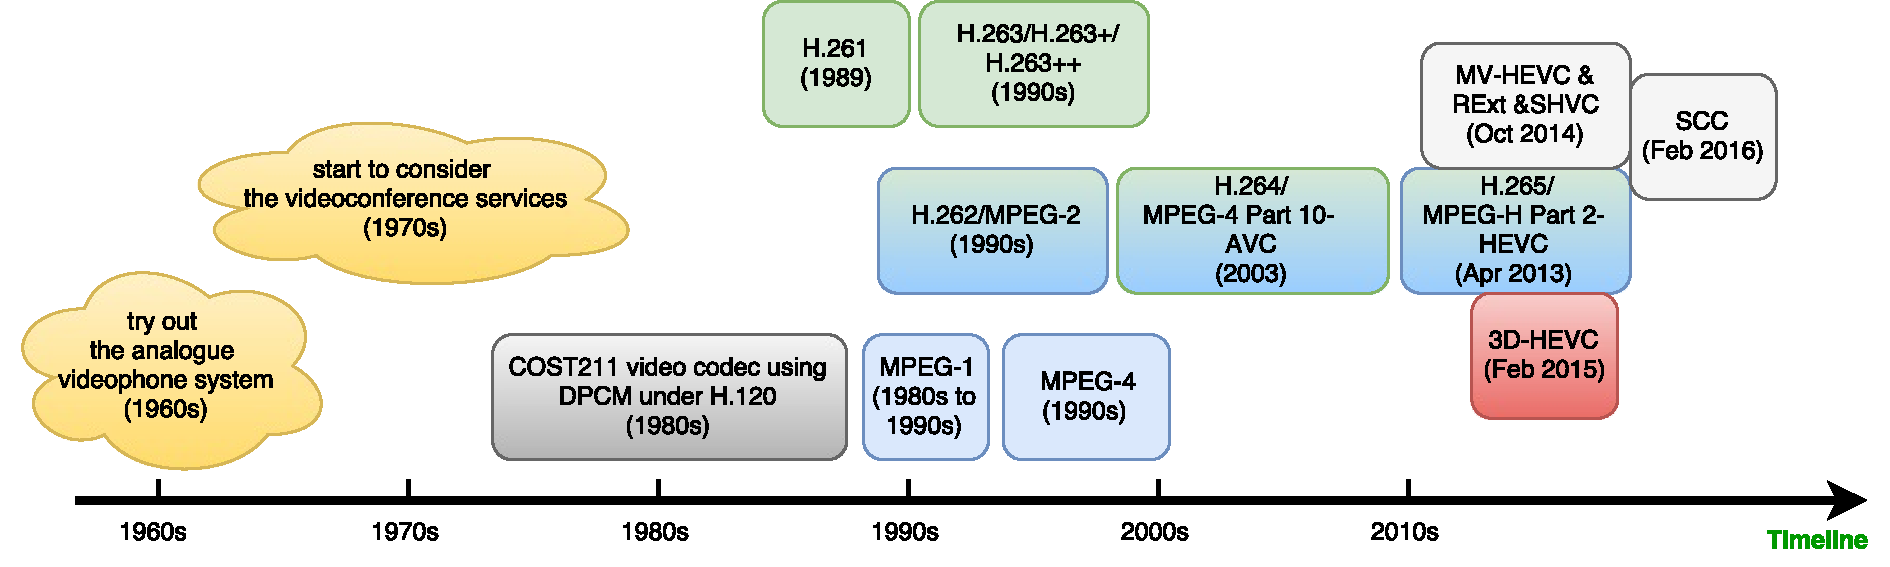
\includegraphics[width=\textwidth,height=\textheight,keepaspectratio]{Figures/video-std-brief-history.pdf}
%        \decoRule
    \caption[The brief history of the video coding standards]
    {The brief history of the video coding standards}
    \label{fig:video-std-brief-history}
\end{figure}
In 1980s, the COST211 video codec, built on top of Differential
Pulse Code Modulation (DPCM), was standardized under H.120 standard by CCITT
(now known as ITU-T).
In late 1989, the H.261 was completed and its success marked a milestone for
video coding at low bit rate with fairly good quality~\parencite{RN181}.
The Motion Picture Experts Group (MPEG) kicked off the exploration of video
storage, such as CD-ROMs.
Their objective was to achieve a competitive performance with cassette
recorders in terms of compression of videos which have rich motions.
The framework of H.261 had been used to start the codec design of MPEG-1.
MPEG-2 was one generation after the MPEG-1.
It featured higher capabilities when handling videos with
high bit rates and high resolutions.
In MPEG-2, the encoder is allowed to make its own decision on the
the number of bi-directionally predicted pictures according to a
suitable coding delay.
ITU-T found this technique applicable to telecommunication applications, as
a result MPEG-2 has been adopted as H.262 for telecommunications.
Right after the MPEG-2 standard, MPEG-3 was designed mainly for coding of
high definition videos.
However, MPEG-3 was discarded due to the versatility of MPEG-2, which
can be used to encode videos of any resolutions.
In the late 1998, MPEG-4 was introduced as a way of defining compression of
both audio and visual digital data.
Later on MPEG-4 was divided into several parts during its continuously evolving.
Among its sub-parts, MPEG-4 part 10 (a.k.a. Advanced Video Coding) is mainly
for the video compression.
With the rising popularity of the high definition videos, the new standard
termed High Efficiency Video Coding (HEVC) for compressing videos in a more
efficient way comparing with previous standards, such as H.264/AVC, has
emerged under the efforts from the Joint Collaborative Team on Video
Coding (JCT-VC).
In the meanwhile, five extensions of the HEVC standard, comprising
Format Range Extension (RExt), Scalability Extension (SHVC),
Multi-view Extension (MV-HEVC), 3D Extension (3D-HEVC),
Screen Content Coding Extension (SCC),  have been finalized
from 2014 to 2016 to fulfill extra requirements in various video coding
scenarios.

In this work, we focus on the depth map coding in 3D-HEVC\@.
The 35 angular modes and depth modeling modes have been embraced in the
depth map coding tools in 3D-HEVC\@.
The DMM1 mode introduces an huge increase for the encoding time of 3D videos.
Acceleration of the depth map coding is needed.

\section{Deep Learning}\label{sec:deep-learning}
Deep learning is an approach of representation learning
(a.k.a. feature learning), which is essentially a method to
learn from data.
Numerous layers of computational units together with appropriate activating
mechanism comprise the basic architecture for deep learning.
Multitudinous data sets are needed for those computational architectures
to learn data abstractions for tasks such as image classification,
speech recognition, object detection, etc.
Each layer learns a level of abstraction from the data sets using
back-propagation algorithm~\parencite{RN204}.
Making use of those learned abstractions, the computational architectures are
able to solve complex problems which are typically non-linear and normally hard
to solve by using specific rules that are designed in advance.

Deep learning has been attracting wide attention from all over the world
in recent years, not only because of the great achievements it has
made in various application scenarios, but also due to the promise of an
intelligent future it gives.
Such a learning methodology makes people believe it is possible
for the formation of wise machines
that they have long dreamed to possess.
The growing data accessibility provides rich examples for deep computational
architectures to adjust their internal weights and bias until their
predictions have low error rate.
On the other hand, the computational devices are relatively
affordable than in the previous years by the society, with the help of which,
accelerations of learning processes has been achieved, hence a bunch of
time consuming deep learning architectures can be tried within acceptable
periods.

In the ILSVRC-2012 competition~\parencite{RN205}, AlexNet~\parencite{RN65}
received the championship with the 15.3\% top-5 error rate, compared to
26.2\% achieved by the runner-up.
Such a large margin of error rate claimed a breakthrough in
object recognition history.
It kicked off a blistering pace of trying out deep learning by both academia
and industry, which in turn led to an increase of the convolutional
neural networks' submissions to ILSVRC-2013, in which ZF Net~\parencite{RN66}
was the winner.
It fine-turned the architecture of AlexNet based on the
gorgeous visualizations of trained models.
Both AlexNet and ZF Net are of the same structure which is built up
by simply stacking computational layers while GoogLeNet~\parencite{RN60}
is composed of Inception
modules.
This new architecture was the most successful candidate in ILSVRC-2014.
It has not only set the new height of object recognition but also started to
optimize the computational resources of the network by design.
It consists of 22 layers, which was deeper than all the previous
networks in ILSVRC\@.
However, it is still not deep enough.
In the ILSVRC-2015, Residual Neural Network (ResNet)~\parencite{RN67} with
152 layers won the championships in all the five main tracks.
ResNet introduced a brand new notion into the neural network architecture
named identity mapping.
The shortcut connection in the identity mapping prevents the degradation of
training accuracy when the network goes deeper.
Besides, the converging speed of ResNet is faster than the network built up
with Inception modules when both are of the similar size.

Despite the fact that neural networks built up from Inception modules
converges slower than those built up from ResNet modules, it is still
worth it for a brief review of the valuable insights residing in
the Inception networks.
A typical incarnation of the first generation of Inception networks is named
GoogLeNet~\parencite{RN60}.
It was intricately carved with a responsibility to win computer vision
tasks in ILSVRC-2014, on which it performed better than all the other
deep neural network architectures.
There exist philosophical reflections which are intend to serve as guidelines
for the construction of Inception networks.
Two major downsides of a enlarged neural network have been discussed
in~\parencite{RN60}.
One is the higher chances of overfitting while the other is
the strikingly increased requirements of computational resources with the
enlarged network size.
For handling those drawbacks, based on the new ideas which were introduced
in~\parencite{RN207} about how to construct the reasonable architecture of
neural networks, new experiments orienting sparse network structure have
been tried out.
One year later after GoogleNet stolen the show in 2014,



% ====== can be used for literature review =====
%AlexNet contains five convolutional layers and three fully-connected
%layers.
%The Rectified Linear Units (ReLU)~\parencite{RN206}, Local Response
%Normalization and Overlapping Pooling were adopted.
%The methodology of multiple GPU training was used to make the learning fast.
%Data Augmentation and Dropout were chosen to overcome the problem of
%Overfitting.
%Stochastic gradient descent was adopted.
% ====== can be used for literature review =====




%Welcome to this \LaTeX{} Thesis Template, a beautiful and easy to use template for writing a thesis using the \LaTeX{} typesetting system.
%
%If you are writing a thesis (or will be in the future) and its subject is technical or mathematical (though it doesn't have to be), then creating it in \LaTeX{} is highly recommended as a way to make sure you can just get down to the essential writing without having to worry over formatting or wasting time arguing with your word processor.
%
%\LaTeX{} is easily able to~\parencite{RN93} professionally typeset documents that run to hundreds or thousands of pages long. With simple mark-up commands, it automatically sets out the table of contents, margins, page headers and footers and keeps the formatting consistent and beautiful. One of its main strengths is the way it can easily typeset mathematics, even \emph{heavy} mathematics. Even if those equations are the most horribly twisted and most difficult mathematical problems that can only be solved on a super-computer, you can at least count on \LaTeX{} to make them look stunning.
%
%%----------------------------------------------------------------------------------------
%
%\section{Welcome and Thanku}\label{sec:welome}
%Welcome to this \LaTeX{} Thesis Template, a beautiful and easy to use template for writing a thesis using the \LaTeX{} typesetting system.
%
%If you are writing a thesis (or will be in the future) and its subject is technical or mathematical (though it doesn't have to be), then creating it in \LaTeX{} is highly recommended as a way to make sure you can just get down to the essential writing without having to worry over formatting or wasting time arguing with your word processor.
%
%\LaTeX{} is easily able to professionally typeset documents that run to hundreds or thousands of pages long. With simple mark-up commands, it automatically sets out the table of contents, margins, page headers and footers and keeps the formatting consistent and beautiful. One of its main strengths is the way it can easily typeset mathematics, even \emph{heavy} mathematics. Even if those equations are the most horribly twisted and most difficult mathematical problems that can only be solved on a super-computer, you can at least count on \LaTeX{} to make them look stunning.
%
%%----------------------------------------------------------------------------------------
%
%\section{Welcome and ThYou}\label{sec:weome}
%Welcome to this \LaTeX{} Thesis Template~\parencite{Reference1}, a beautiful and easy to use template for writing a thesis using the \LaTeX{} typesetting system.
%
%If you are writing a thesis (or will be in the future) and its subject is technical or mathematical (though it doesn't have to be), then creating it in \LaTeX{} is highly recommended as a way to make sure you can just get down to the essential writing without having to worry over formatting or wasting time arguing with your word processor.
%
%\LaTeX{} is easily able to professionally typeset documents that run to hundreds or thousands of pages long. With simple mark-up commands, it automatically sets out the table of contents, margins, page headers and footers and keeps the formatting consistent and beautiful. One of its main strengths is the way it can easily typeset mathematics, even \emph{heavy} mathematics. Even if those equations are the most horribly twisted and most difficult mathematical problems that can only be solved on a super-computer, you can at least count on \LaTeX{} to make them look stunning.
%
%%----------------------------------------------------------------------------------------
%
%\section{Welcome and Thau}\label{sec:welcoe}
%Welcome to this \LaTeX{} Thesis Template, a beautiful and easy to use template for writing a thesis using the \LaTeX{} typesetting system.
%
%If you are
%\begin{table}
%
%    \label{tab:treatments}
%    \centering
%%    \begin{tabular}{l l l}
%%        \toprule
%%        \tabhead{Groups} & \tabhead{Treatment X} & \tabhead{Treatment Y} \\
%%        \midrule
%%        1 & 0.2 & 0.8\\
%%        2 & 0.17 & 0.7\\
%%        3 & 0.24 & 0.75\\
%%        4 & 0.68 & 0.3\\
%%        \bottomrule\\
%%    \end{tabular}
%    \begin{tabular}{c r @{.} l}
%        Pi expression       &
%        \multicolumn{2}{c}{Value} \\
%        \hline
%        $\pi$               & 3&1416  \\
%        $\pi^{\pi}$         & 36&46   \\
%        $(\pi^{\pi})^{\pi}$ & 80662&7 \\
%    \end{tabular}
%    \caption{The effects of treatments X and Y on the four groups studied.}
%\end{table}
%writing a thesis (or will be in the future) and its subject is technical or mathematical (though it doesn't have to be), then creating it in \LaTeX{} is highly recommended as a way to make sure you can just get down to the essential writing without having to worry over formatting or wasting time arguing with your word processor.
%
%\LaTeX{} is easily able to professionally typeset documents that run to hundreds or thousands of pages long. With simple mark-up commands, it automatically sets out the table of contents, margins, page headers and footers and keeps the formatting consistent and beautiful. One of its main strengths is the way it can easily typeset mathematics, even \emph{heavy} mathematics. Even if those equations are the most horribly twisted and most difficult mathematical problems that can only be solved on a super-computer, you can at least count on \LaTeX{} to make them look stunning.
%
%%----------------------------------------------------------------------------------------
%
%\section{Welcome and Tnk You}\label{sec:wlcome}
%Welcome to this \LaTeX{} Thesis Template, a beautiful and easy to use template for writing a thesis using the \LaTeX{} typesetting system.
%
%If you are writing a thesis.
%
%%\begin{verbatim}
%\begin{figure}
%    \centering
%    
\includegraphics{Figures/Electron}
%    %    \decoRule
%    \caption[An Electron]{An electron (artist's impression).}
%    \label{fig:Electron}
%\end{figure}
%%\end{verbatim}
%(or will be in the future) and its subject is technical or mathematical (though it doesn't have to be), then creating it in \LaTeX{} is highly recommended as a way to make sure you can just get down to the essential writing without having to worry over formatting or wasting time arguing with your word processor.
%
%\LaTeX{} is easily able to professionally typeset documents that run to hundreds or thousands of pages long. With simple mark-up commands, it automatically sets out the table of contents, margins, page headers and footers and keeps the formatting consistent and beautiful. One of its main strengths is the way it can easily typeset mathematics, even \emph{heavy} mathematics. Even if those equations are the most horribly twisted and most difficult mathematical problems that can only be solved on a super-computer, you can at least count on \LaTeX{} to make them look stunning.
%
%%----------------------------------------------------------------------------------------
%    \chapter{Conclusions}
    ...
%    \appendix
%    \chapter{A Long Proof}
    ...
    \printbibliography[heading=bibintoc]
\end{document}